\documentclass[a4paper,12pt]{article}
%For images
\usepackage{graphicx}
 
\addtolength{\oddsidemargin}{-.875in}
\addtolength{\evensidemargin}{-.875in}
\addtolength{\textwidth}{1.75in}
 
\addtolength{\topmargin}{-.875in}
\addtolength{\textheight}{1.75in}
 
\begin{document}
\begin{enumerate}
    \item I uppgiften görs ett antagande att den även begränsas
    av y-axeln.

    \begin{center}
        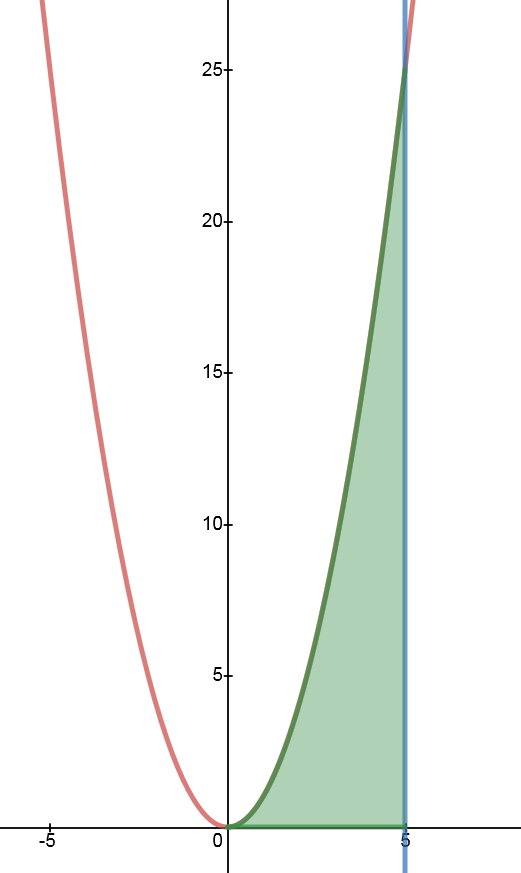
\includegraphics[scale=0.4]{Figur 1.png}
    \end{center}

    Eftersom rotationen sker kring x-axeln så blir
    värdet på y radien, och då används formeln
    $$\pi\int_a^bf(x)^2dx$$
    I figuren så kan man observera att integralen går från 0 till 5
    $$\pi\int_0^5(x^2)^2dx=\pi\int_0^5x^4dx$$
    Som då integreras
    $$\Rightarrow \pi(\frac{x^5}{5})]^5_0=\pi 5^5/5=\pi 625 v.e$$

    \item Radien i denna uppgift blir istället radien x. Då hamnar x på $x=y^2$.
    Vilket grafiskt kan tänkas som att funktionerna $x^2$ och $\sqrt{x}$ har en rotationel
    symetri. Då används formeln 
    $$\pi\int_a^bf(y)^2dy$$
    \begin{center}
        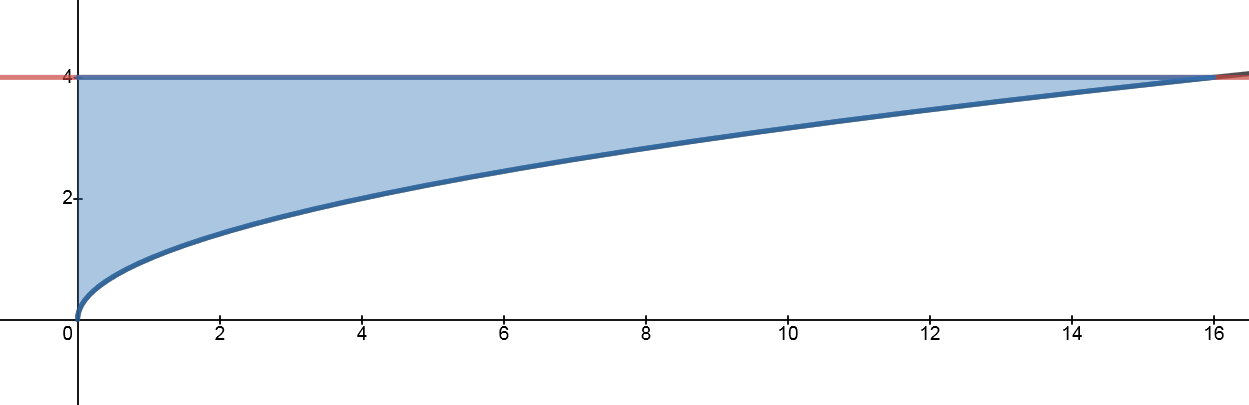
\includegraphics[scale=0.4]{Figur 2.png}
    \end{center}
    
    I figuren ser vi att integralen går från 0 till 4.
    $$\pi\int_0^4(y^2)^2dy=\pi\int_0^4y^4dy$$
    $$\Rightarrow \pi\frac{y^5}{5}]^4_0=\pi \frac{4^5}{5}=\pi \frac{1024}{5} v.e$$


    \item Följande area ska utberäknas
    \begin{center}
        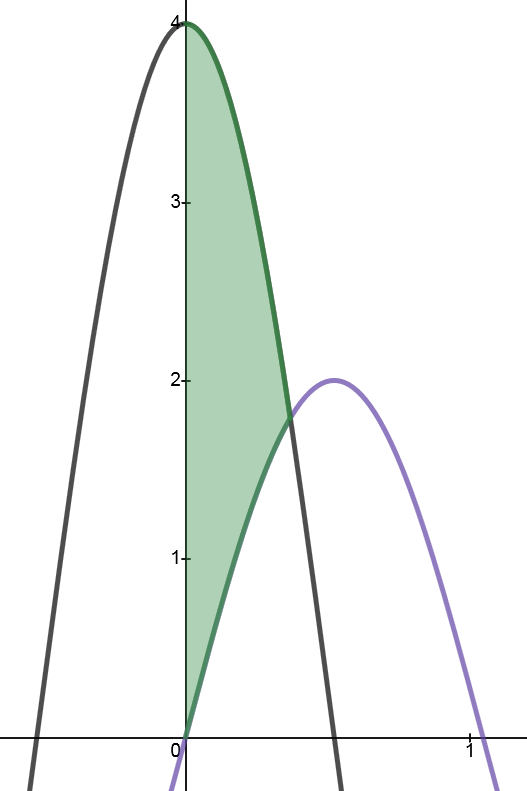
\includegraphics[scale=0.4]{Figur 3.png}
    \end{center}

    Med sådana integraler räknar man rektanglarna mellan funktionerna, dvs
    $g(x)-f(x)$, och integrerar sedan över den nya funktionen som i detta
    fall blir $$4cos(3x)-2sin(3x)$$

    Som då blir den här arean
    \begin{center}
        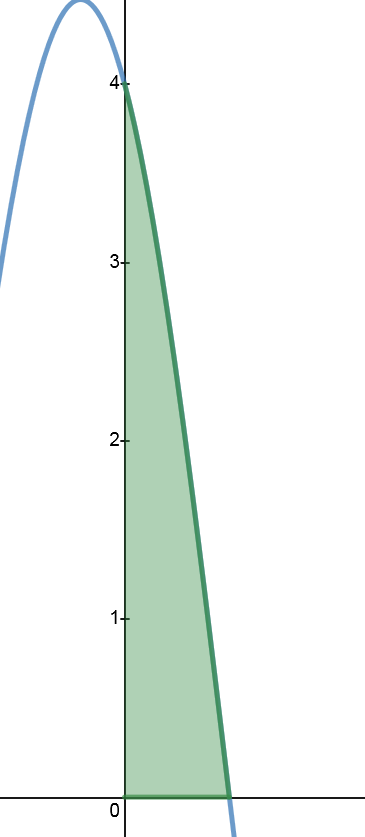
\includegraphics[scale=0.4]{Figur 4.png}
    \end{center}

    Integralen som räknas ut blir då mellan 0 och intersektionspunkten.
    Intersektionspunkten är när 
    $$4cos(3x)=2sin(3x)\Rightarrow 2=\frac{sin(3x)}{cos(3x)}=tan(3x)\Rightarrow x=\frac{tan^{-1}(2)}{3}$$
    
    $$\int_0^{tan^{-1}(2)/3}4cos(3x)-2sin(3x)dx=\frac{4sin(3x)+2cos(3x)}{3}]^{tan^{-1}(2)/3}_0$$
    $$=\frac{4sin(tan^{-1}(2))+2cos(tan^{-1}(2))-2}{3}\approx \frac{4sin(1.11)+2cos(1.11)-2}{3}\approx 0.824 a.e$$

    Detta är rimligt med tanke på att området är väldigt tunt.

    \item Differentialekvationen kan skrivas om som $y'=-3y$. Som då kan integreras och lösas ut som
    $${dx}=\frac{1}{-3y}dy\Rightarrow x=-\frac{1}{3}ln(y)+C$$

    Funktionen den här bildar är väldigt lik en bakvänd $e^x$ funktion
    \begin{center}
        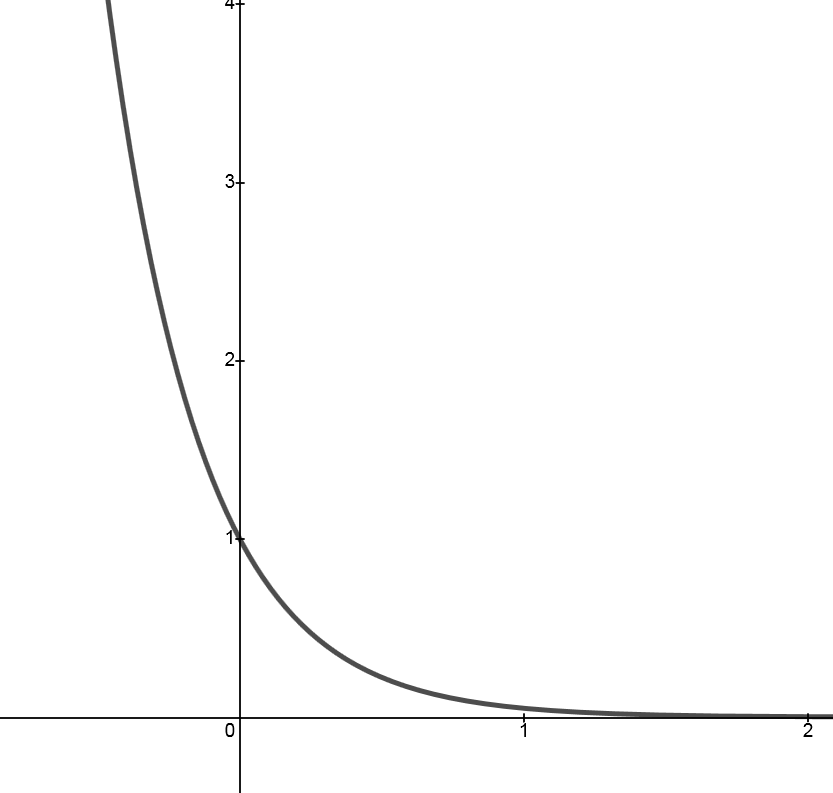
\includegraphics[scale=0.4]{Figur 5.png}
    \end{center}

    Löser man ut y får man ekvationen.

    $$x-C=-\frac{1}{3}ln(y)\Rightarrow 3C-3x=ln(y)\Rightarrow y=e^{3c-3x}$$
    Antar man att c=0 så blir konstanten $a=-3$.

    \item 

    $$sin(x) + \frac{cos(2x)}{2}]_0^{\pi/2}$$
    $$=1-1/2-1/2=0$$

    Man kan verifiera det här grafiskt
    \begin{center}
        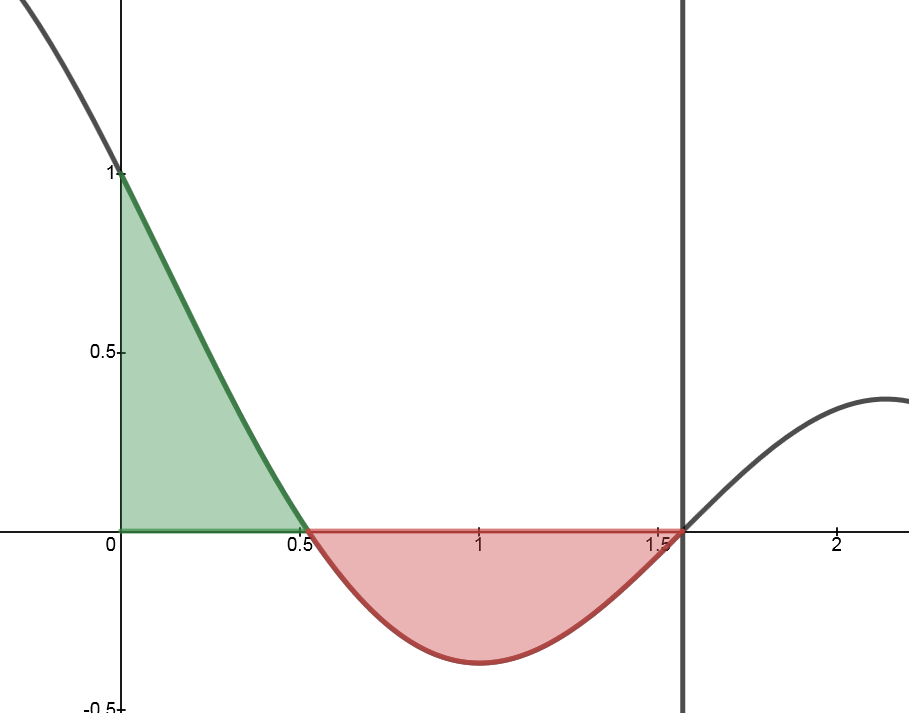
\includegraphics[scale=0.4]{Figur 8.png}
    \end{center}

    Man kan uppmana att den gröna arean minus den röda arean
    kommer ligga välidigt nära noll då dom, med ögonmått, ser
    ut att vara lika stora.

    \item Man kan sätta in lösningen i den originella differnetialekvationen.
    
    $$y'=A-2B/x^3$$
    $$y''=6B/x^4$$

    Sedan sätts dom in i ekvationen.

    $$x^2 6B/x^4+2x(A-2B/x^3)-2(Ax+B/x^2)$$
    $$=6B/x^2+2xA-4B/x^2-2xA-2B/x^2$$
    $$=\frac{B}{x^2}(6-4-2)+2xA(2-2)$$
    $$=0$$

    Vilket är korrekt enligt uppgiften.
    
    \item Följande områden ska bilda rotationsvolymer där area A är lila
    och area B är röd. 
    \begin{center}
        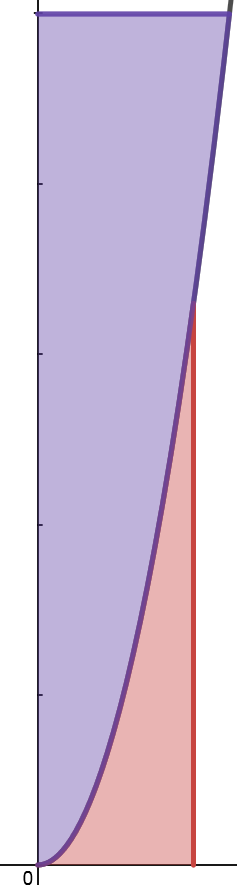
\includegraphics[scale=0.4]{Figur 6.png}
    \end{center}

    Där den lila linjen visar vart y=b är och den röda linjen
    visar vart x=a är. Rotationsvolymen $V_a$ roterar på x-axeln och går
    mellan 0 och a, så då blir det $V_a=\pi\int_0^ax^4dx$ medans för den som
    roterar runt y axeln blir $V_b=\pi\int_0^bydy$. Sambadet mellan dom räknas
    då ut som följande.

    $$\pi\int_0^ax^4dx=\pi\int_0^bydy\Rightarrow \frac{x^5}{5}]_0^a=\frac{y^2}{2}]_0^b\Rightarrow \frac{a^5}{5}=\frac{b^2}{2}\Rightarrow 2a^5=5b^2$$
    $$\Rightarrow b=\sqrt{\frac{2a^5}{5}}=\frac{\sqrt{2}}{\sqrt{5}}a^{5/2}$$

    Enligt ekvationen åvan, vid större värden av a, så måste b växa
    väldigt fort. Detta är logiskt då rotationsvolymen som bildas
    av b (den lila delen av bilden nedan) växer mycket långsammare 
    än den som är begränsad av a (röda delen). En liten förändring
    db bildar en mycket större förändring da. 

    \begin{center}
        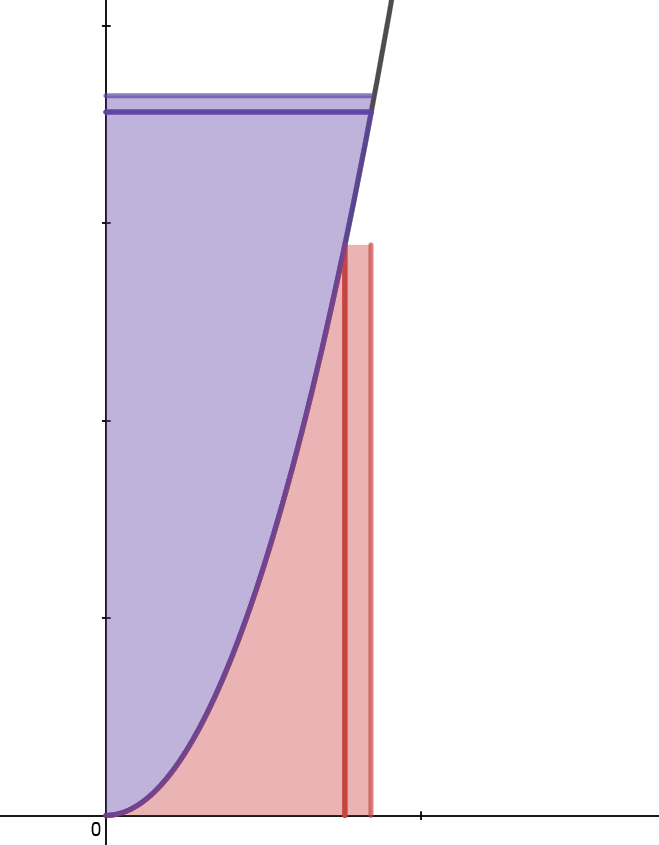
\includegraphics[scale=0.35]{Figur 7.png}
    \end{center}


\end{enumerate}
\end{document}